\documentclass{article}
\usepackage{amsmath}
\usepackage{enumerate}
\usepackage{fancyhdr} % Required for custom headers
\usepackage{lastpage} % Required to determine the last page for the footer
\usepackage{extramarks} % Required for headers and footers
\usepackage[usenames,dvipsnames]{color} % Required for custom colors
\usepackage{graphicx} % Required to insert images
\usepackage[tight,footnotesize]{subfigure} % Required for subfig
\usepackage{caption} % Required for subfig
\usepackage{hyperref} % Required for url
\usepackage{listings} % Required for insertion of code
\usepackage{courier} % Required for the courier font
\usepackage{lipsum} % Used for inserting dummy 'Lorem ipsum' text into the template
\topmargin=-0.45in
\evensidemargin=0in
\oddsidemargin=0in
\textwidth=6.5in
\textheight=9.0in
\headsep=0.25in
\linespread{1.1} % Line spacing
\pagestyle{fancy}
\lhead{\hmwkAuthorName} % Top left header
% \chead{\hmwkClass\ (\hmwkClassInstructor\ \hmwkClassTime): \hmwkTitle} % Top center head
\chead{\hmwkClass\ : \hmwkTitle} % Top center head
\rhead{\firstxmark} % Top right header
\lfoot{\lastxmark} % Bottom left footer
\cfoot{} % Bottom center footer
\rfoot{Page\ \thepage\ of\ \protect\pageref{LastPage}} % Bottom right footer
\renewcommand\headrulewidth{0.4pt} % Size of the header rule
\renewcommand\footrulewidth{0.4pt} % Size of the footer rule
\setlength\parindent{0pt} % Removes all indentation from paragraphs

% Define floor and ceiling
\def\lc{\left\lceil}   
\def\rc{\right\rceil}
\def\lf{\left\lfloor}   
\def\rf{\right\rfloor}

% Set your language 
%\lstset{language=Java}
\definecolor{codegreen}{rgb}{0,0.6,0}
\definecolor{codegray}{rgb}{0.5,0.5,0.5}
\definecolor{codepurple}{rgb}{0.58,0,0.82}
\definecolor{backcolour}{rgb}{0.95,0.95,0.92}
 
\lstdefinestyle{mystyle}{
    backgroundcolor=\color{backcolour},   
    commentstyle=\color{codegreen},
    keywordstyle=\color{magenta},
    numberstyle=\tiny\color{codegray},
    stringstyle=\color{codepurple},
    basicstyle=\footnotesize,
    breakatwhitespace=false,         
    breaklines=true,                 
    captionpos=b,                    
    keepspaces=true,                 
    numbers=left,                    
    numbersep=8pt,                  
    showspaces=false,                
    showstringspaces=false,
    showtabs=false,                  
    tabsize=2
}
\lstset{style=mystyle}

% Header and footer for when a page split occurs within a problem environment
\newcommand{\enterProblemHeader}[1]{
\nobreak\extramarks{#1}{#1 continued on next page\ldots}\nobreak
\nobreak\extramarks{#1 (continued)}{#1 continued on next page\ldots}\nobreak
}

% Header and footer for when a page split occurs between problem environments
\newcommand{\exitProblemHeader}[1]{
\nobreak\extramarks{#1 (continued)}{#1 continued on next page\ldots}\nobreak
\nobreak\extramarks{#1}{}\nobreak
}

\setcounter{secnumdepth}{0} % Removes default section numbers
\newcounter{homeworkProblemCounter} % Creates a counter to keep track of the number of problems

\newcommand{\homeworkProblemName}{}
\newenvironment{homeworkProblem}[1][Problem \arabic{homeworkProblemCounter}]{ % Makes a new environment called homeworkProblem which takes 1 argument (custom name) but the default is "Problem #"
\stepcounter{homeworkProblemCounter} % Increase counter for number of problems
\renewcommand{\homeworkProblemName}{#1} % Assign \homeworkProblemName the name of the problem
\section{\homeworkProblemName} % Make a section in the document with the custom problem count
\enterProblemHeader{\homeworkProblemName} % Header and footer within the environment
}{
\exitProblemHeader{\homeworkProblemName} % Header and footer after the environment
}

\newcommand{\problemAnswer}[1]{ % Defines the problem answer command with the content as the only argument
\noindent\framebox[\columnwidth][c]{\begin{minipage}{0.98\columnwidth}#1\end{minipage}} % Makes the box around the problem answer and puts the content inside
}

\newcommand{\homeworkSectionName}{}
\newenvironment{homeworkSection}[1]{ % New environment for sections within homework problems, takes 1 argument - the name of the section
\renewcommand{\homeworkSectionName}{#1} % Assign \homeworkSectionName to the name of the section from the environment argument
\subsection{\homeworkSectionName} % Make a subsection with the custom name of the subsection
\enterProblemHeader{\homeworkProblemName\ [\homeworkSectionName]} % Header and footer within the environment
}{
\enterProblemHeader{\homeworkProblemName} % Header and footer after the environment
}

\newlength{\tabcont}

\newcommand{\tab}[1]{%
\settowidth{\tabcont}{#1}%
\ifthenelse{\lengthtest{\tabcont < .25\linewidth}}%
{\makebox[.25\linewidth][l]{#1}\ignorespaces}%
{\makebox[.5\linewidth][l]{\color{red} #1}\ignorespaces}%
}%
%----------------------------------------------------------------------------------------
%	NAME AND CLASS SECTION
%----------------------------------------------------------------------------------------

\newcommand{\hmwkTitle}{Homework\ \#6} % Assignment title
\newcommand{\hmwkDueDate}{Monday,\ January\ 1,\ 2012} % Due date
\newcommand{\hmwkClass}{Fundamental Algorithms} % Course/class
\newcommand{\hmwkClassTime}{} % Class/lecture time
\newcommand{\hmwkClassInstructor}{Prof. Joel Spencer} % Teacher/lecturer
\newcommand{\hmwkAuthorName}{Songxiao Zhang, N10224459, {\tt 72}} % Your name

%----------------------------------------------------------------------------------------
%	TITLE PAGE
%----------------------------------------------------------------------------------------

\title{
\textmd{\textbf{\hmwkClass:\ \hmwkTitle}}\\
}
\author{\textbf{\hmwkAuthorName}}

\begin{document}

\maketitle

%----------------------------------------------------------------------------------------
%	PROBLEM 1
%----------------------------------------------------------------------------------------
\begin{homeworkProblem}
\begin{enumerate}[(a)]
    \item f. Find the successor is to find the $MIN$ of right sub-tree since all the keys in the 
          right sub-tree are larger than the key of c. \\
          The $MIN$ of a tree is the left-most item. \\
          c.right = g, g.left = f, f.left = NIL so return f. 
          
\begin{lstlisting}[frame=single]
SUCCESSOR (n)
    return MIN(n.right)
\end{lstlisting}

          
    \item h. As mentioned above, the $MIN$ of a tree is the left-most item.\\
          ROOT[T].left = a.left = h, h.left = NIL so return h. 
          
\begin{lstlisting}[frame=single]
MIN (n)
    while(n.left != NIL)
        n = n.left
    return n
\end{lstlisting}
            
          
    \item In the subtree of Tree(e.parent) = Tree(d), d.left = e, d.right = NIL, 
          e.left = c, e.right = b, c.left = NIL, c.right = g, g and b are leaves. \\
          Since c has child(ren) and d is childless, we can DELETE[e] by move up d. 
          That is d.left = b, b.left = c, c.parent = b. 
          
\begin{lstlisting}[frame=single]
DELETE(n, val) {
    if (val < n.value) {
          if (n.left != null)
                return n.left.remove(val, n);
          else
                return false;
    } else if (val > n.value) {
          if (n.right != null)
                return n.right.remove(val, n);
          else
                return false;
    } else {
        if (n.left != null && n.right != null) {
            n.value = n.right.MIN();
            n.right.DELETE(n.value, n);
        } else if (n.parent.left == n) {
            n.parent.left = (n.left != null) ? n.left : n.right;
        } else if (parent.right == this) {
            n.parent.right = (n.left != null) ? n.left : n.right;
        }
    }
}
\end{lstlisting}
\end{enumerate}
\end{homeworkProblem}

%----------------------------------------------------------------------------------------
%	PROBLEM 2
%----------------------------------------------------------------------------------------
\begin{homeworkProblem}
There is a trick doing this question: when constructing a fully balanced binary tree, pick 
the node with its key is the medium value as the root, then doing the same in the branches
until all the nodes are covered. Now we can get the tree with the lowest height $O(\lceil lgN \rceil)$. The results are shown in Figure~\ref{fig:flow} on Page~\pageref{fig:flow}.

\begin{figure}[!h]
        \centering
        \subfigure[]{\label{}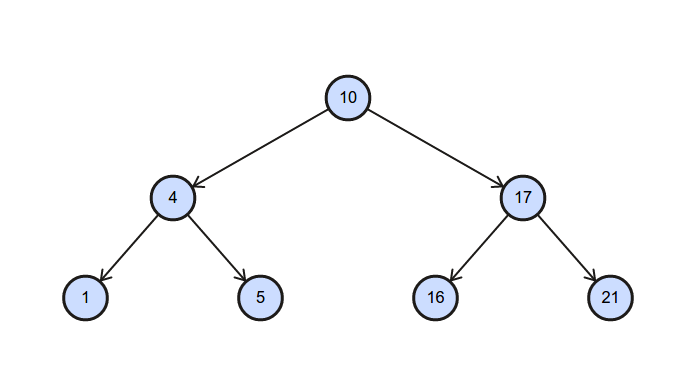
\includegraphics[scale=0.22]{hw6/2.png}}
        \subfigure[]{\label{}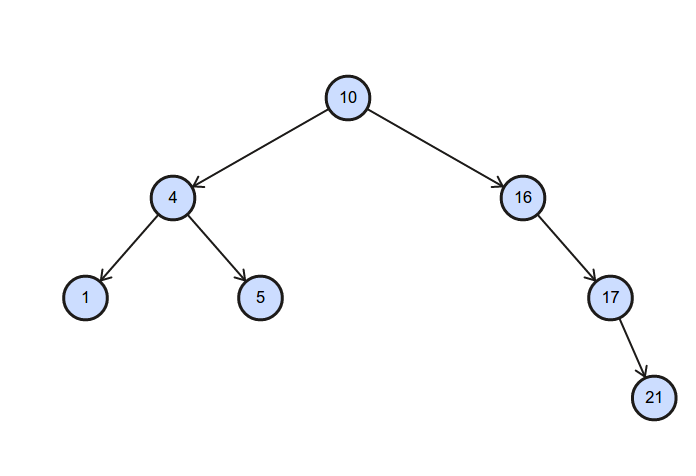
\includegraphics[scale=0.22]{hw6/3.png}}
        \subfigure[]{\label{}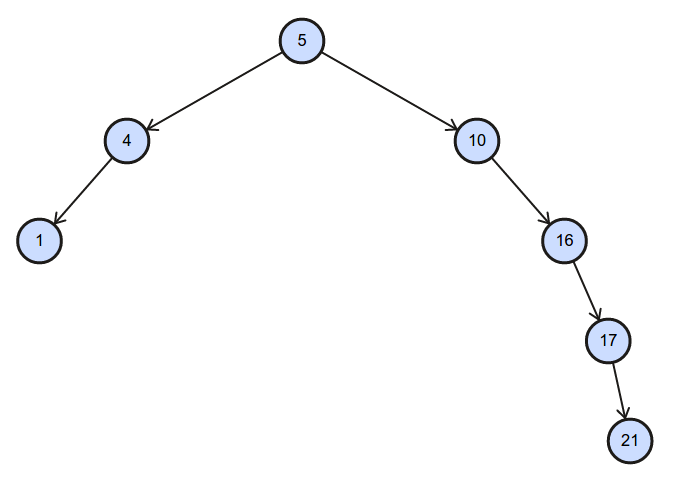
\includegraphics[scale=0.22]{hw6/4.png}}
        \subfigure[]{\label{}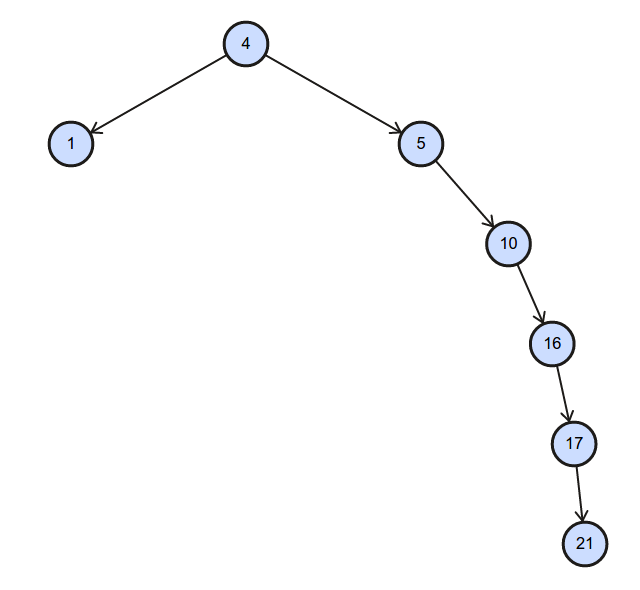
\includegraphics[scale=0.25]{hw6/5.png}}
        \subfigure[]{\label{}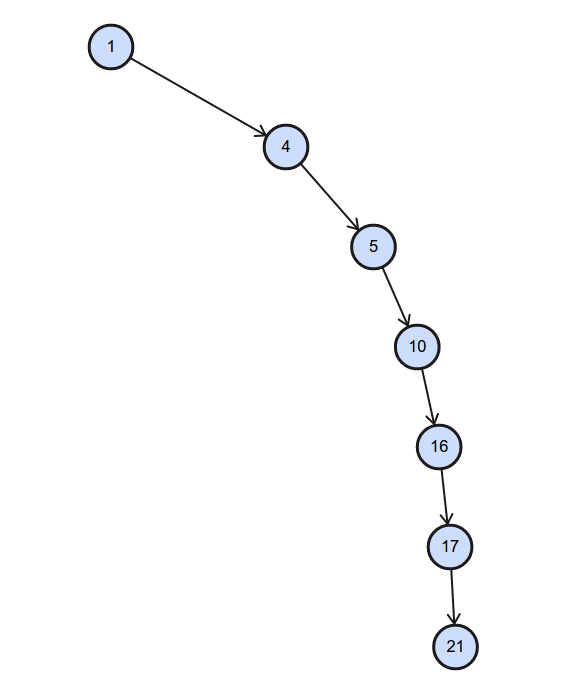
\includegraphics[scale=0.25]{hw6/6.png}}
        \caption{The easiest and most intuitive way to draw the tree set I found is switching the root (a to e are BST of heights 2 to 6)}
        \label{fig:flow}
    \end{figure} 
    
\end{homeworkProblem}

%----------------------------------------------------------------------------------------
%	PROBLEM 3
%----------------------------------------------------------------------------------------
\begin{homeworkProblem}
Max-Heap: For any node $n$, $n.value > n.left.value$, $n.value > n.right.value$ \\
BST: For any node $n$, $n.value > n.left.value$, $n.value < n.right.value$ \\
It's not possible. To print the tree in sorted order, all elements need to be sorted first. 
With heap-property, HeapSort takes $O(nlgn)$ so cannot finish in $O(n)$. 
\end{homeworkProblem}

%----------------------------------------------------------------------------------------
%	PROBLEM 4
%----------------------------------------------------------------------------------------
\begin{homeworkProblem}
This question is similar to using a HashMap checking duplicates. We can put the hash values of elements from A in the table every time after checking whether there's something already in that index. The running time is $\Theta(N)$. \\

But we need to take care of hash collision, i.e., 2 different input returned the same hash value but we shouldn't call it duplicate. So we cannot only store the hash value but the original value also in order to check whether there's a collision. In this question, since the length of the table is the same as the hashtable size, we can take the table index indicating the hash value. When there's collision, check whether it is a duplicate; if not, don't insert the value as we're not required to fill all elements of A into T. \\

Here, I provide the python code for this algorithm: 
\begin{lstlisting}[frame=single]
# python code
BAD = 0
GOOD = 1
def findDuplicate(T, A):
	for i in range(0, n):
		# check dup; handle hash collision
		if T.index(hash(A[i])) != None and A[i] != T.index(hash(A[i])):
			return BAD;
		else T.insert(i, hash(A[i]))
	return GOOD
		
// java code
static final int BAD = 0;
static final int GOOD = 1;
public int findDuplicate(List T, int[] A) {
	HashMap<Integer, String> hm = new HashMap<Integer, String>(T);
	for (int i = 0; i < n; i++) {
		// check dup; handle hash collision
		if (hm.get(hash(A[i])) != null and hm.get(A[i]) != A[i])
			return BAD;
		else hm.put(A[i]);
	}
	return GOOD;
}
\end{lstlisting}

\end{homeworkProblem}

%----------------------------------------------------------------------------------------
%	PROBLEM 5
%----------------------------------------------------------------------------------------
\begin{homeworkProblem}
Stick to the BST property: a.left.value < a.value < a.right.value. An sorted decreasing array would be always appended at the left side. An sorted increasing array would be always appended at the right side. Show in Figure~\ref{fig:tree} on Page~\pageref{fig:tree}.
    
\begin{figure}[h!]
    \centering
    \subfigure[]{\label{}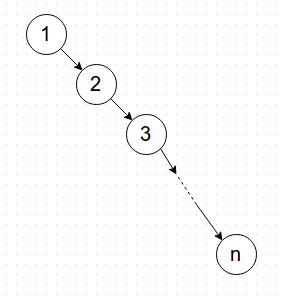
\includegraphics[scale=0.4]{hw6/51.png}}
    \subfigure[]{\label{}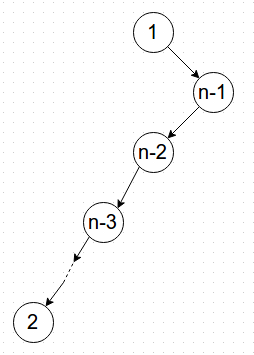
\includegraphics[scale=0.4]{hw6/52.png}}
    \caption{insert an increasingly sorted bst; insert an decreasingly sorted bst}
    \label{fig:tree}
\end{figure} 
    

\end{homeworkProblem}

% \begin{lstlisting}[frame=single]
% \end{lstlisting}

% \begin{enumerate}[a.]
%     \item 
        %   
        %   
% \end{enumerate}
\end{document}